\section{Web Application}
\label{sec:webapp}

Unlike traditional software application that only resides on the operating system we have, web appplication allow users to use a service that is available on the Web.
The application mostly heavily created with JavaScript on the client side and with various languages on the server side whether it is on a platform like Node.js, Ruby, Python, Java, Go, etc.
So a web application can include an application program executing at a web site on a server, and accessible remotely from a user device through a communications network.~\autocite{Addala:2013:InteractiveWebAppFramework}
Example of most popular web applications used by people today are Google, Gmail, Twitter, Facebook, and YouTube.
Within web application architecture, each application can communicate with each other, often with an \ac{API} like REST or even a communication protocol such as WebSocket over the usual standard \ac{HTTP}.
The communication includes the reception and publication of data that has already been processed by any of client or server application.
How a web application usually architected is illustrated in \autoref{fig:webapp}.

\begin{figure}[htbp]
    \centering
    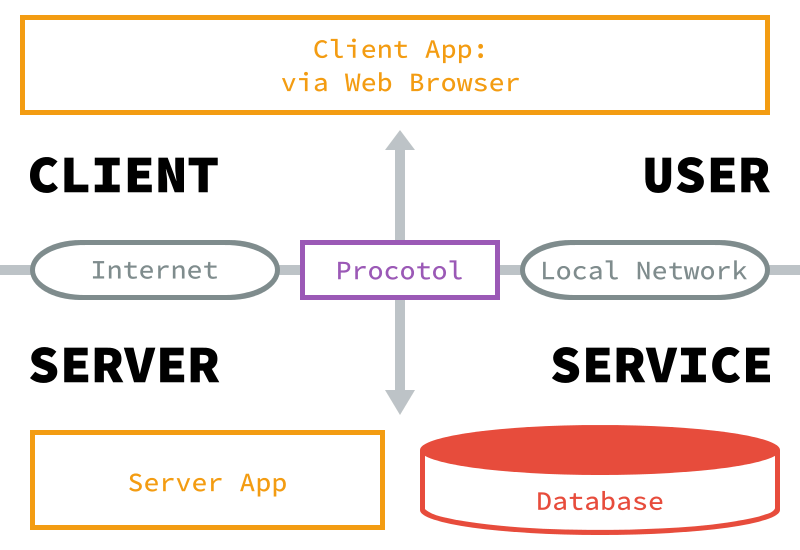
\includegraphics[width=8cm]{\dir/include/webapp.png}
    \caption[Web Application Architecture]{Illustration of a simple web application architecture}
    \label{fig:webapp}
\end{figure}

The application is separated into two main types, a server app and client app that can be a lot of it.
Server app is the service dominantly processes the data and interact directly with the database.
Various data can be transferred over a protocol (often with \ac{HTTP}) via the Internet or even a local network.
The data then received to or sent by the client app which is the user.
It is done by request and respond method if it is using \ac{HTTP}
Or, it can be publish and subscribe method if it is using protocol that has \ac{Pub/Sub} messaging pattern
Majority of the client app are run inside a web browser although sometimes it could be a native software on the desktop or mobile \ac{OS}.
